 \documentclass[12pt]{article}
\setlength\parindent{0pt}
\usepackage{amsmath}
\usepackage{lscape}
\usepackage{graphicx}
\usepackage{fullpage}
\usepackage[margin=0.8in]{geometry}
\setlength{\parskip}{4mm}
\def\LL{\left\langle}   % left angle bracket
\def\RR{\right\rangle}  % right angle bracket
\def\LP{\left(}         % left parenthesis
\def\RP{\right)}        % right parenthesis
\def\LB{\left\{}        % left curly bracket
\def\RB{\right\}}       % right curly bracket
\def\PAR#1#2{ {{\partial #1}\over{\partial #2}} }
\def\PARTWO#1#2{ {{\partial^2 #1}\over{\partial #2}^2} }
\def\PARTWOMIX#1#2#3{ {{\partial^2 #1}\over{\partial #2 \partial #3}} }
\newcommand{\BE}{\begin{displaymath}}
\newcommand{\EE}{\end{displaymath}}
\newcommand{\BNE}{\begin{equation}}
\newcommand{\ENE}{\end{equation}}
\newcommand{\BEA}{\begin{eqnarray}}
\newcommand{\EEA}{\nonumber\end{eqnarray}}
\newcommand{\EL}{\nonumber\\}
\newcommand{\la}[1]{\label{#1}}
\newcommand{\ie}{{\em i.e.\ }}
\newcommand{\eg}{{\em e.\,g.\ }}
\newcommand{\cf}{cf.\ }
\newcommand{\etc}{etc.\ }
\newcommand{\Tr}{{\rm tr}}
\newcommand{\etal}{{\it et al.}}
\newcommand{\OL}[1]{\overline{#1}\ } % overline
\newcommand{\OLL}[1]{\overline{\overline{#1}}\ } % double overline
\newcommand{\OON}{\frac{1}{N}} % "one over N"
\newcommand{\OOX}[1]{\frac{1}{#1}} % "one over X"
\pagenumbering{gobble}

\begin{document}
\Large
\centerline{\sc{Tutorial-Exercise -- The Motion of the Zodiac}}

\normalsize

In this exercise, you'll learn why some constellations appear in the sky at different times of year.

While the entire sky is full of stars, and stargazers have described patterns (constellations) in the whole sky, the most famous are the constellations that lie in the same plane as the Earth's orbit. Since all of the other planets also orbit in this plane, this means that the Sun and the planets travel in the same path in the sky as these constellations.

These are called the {\it Zodiac}. By convention there are twelve of them. We can draw a diagram of Earth's orbit and their locations. 
\begin{center}
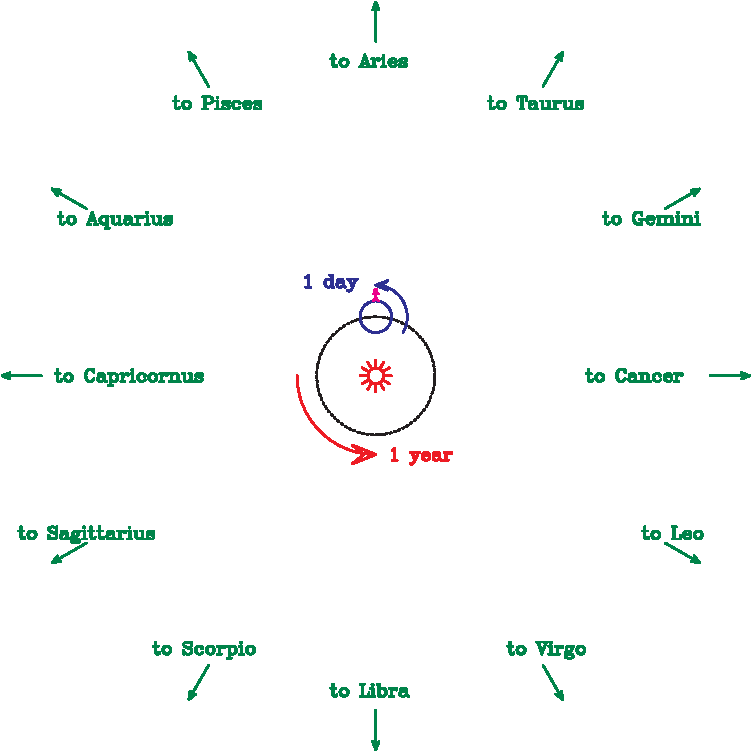
\includegraphics[width=0.8\textwidth]{earth-orbit-crop.pdf}
\end{center}

This is a diagram of the Earth's orbit around the Sun, seen from above the North Pole, with the directions to the (very far away) constellations shown. Note that the Earth rotates counterclockwise, and the Earth revolves around the Sun counterclockwise as well, from this perspective.

Keep in mind that the Earth and Sun are really much smaller than this, and that the Earth's orbit is tiny compared to the distances to the stars.


\newpage

\begin{center}
	Tear the first page off, so you can look at the diagram while answering the questions that follow.
\end{center}
\newpage
\begin{enumerate}
	\item 
Looking at the diagram on the previous page, will an observer on Earth, when it is in the position shown, ever see Libra? {\it (Hint: What will happen to them if they try to look at Libra?)}

\vspace{1in}

\item In the previous page, there is a stick figure drawn on Earth. Since we are looking down from above the North Pole, they are standing on the Equator, with their feet on the ground and their head pointed to the sky. What time of day is it (sunrise, sunset, noon, midnight, etc.) for this person, and how do you know?


\vspace{1in}

\item Many astrological systems describe different times of year by the constellation that is ``behind the Sun''. Even though you cannot see it from the Earth, ancient astronomers were able to figure this out. In the position of the Earth shown, which constellation is lined up with the Sun?

\vspace{1in}

\item Does your answer to the previous question depend on what time of day it is? {\it (Hint: Remember the Earth is very small.)}

\vspace{0.5in}

\item Which two constellations in the Zodiac are lying nearest the observer's horizon?

\vspace{1in}

\item In the previous question, we saw the two constellations lying nearest the horizon. Keeping in mind that the Earth rotates counterclockwise as seen from above, which one is rising in the East and which one is setting in the West?

\newpage

\item Look back at the diagram on the first page. One {\it day} in the future from the time shown, where will the Earth be located? What constellation will be behind the Sun?

\vspace{1in}

\item Now, consider a point in time {\it one month} in the future. Where will the Earth be located in its orbit now? Draw its new position, and draw a stick figure at the location on Earth that is experiencing midnight. 

\vspace{1in}

\item Which constellation will be behind the Sun at this time?

\vspace{1in}

\item At midnight at this time, five constellations will be clearly visible above the horizon. Which are they? Which one has just risen in the East, and which one will be setting in the West? 

\vspace{1in}

\item Which constellation will be the next one to rise?


\newpage


\end{enumerate}



\begin{center}
	\sc \Large Astronomy 101 Homework 2 \\ \large Consequences of the Earth's Orbit\\
	\normalsize \rm Due September 15, when we will have a quiz in class
\end{center}

Here's a diagram of Earth in its current location in orbit, with an observer shown as a stick figure. On the next page, I'll ask you to indicate some things on the diagram.
\begin{center}
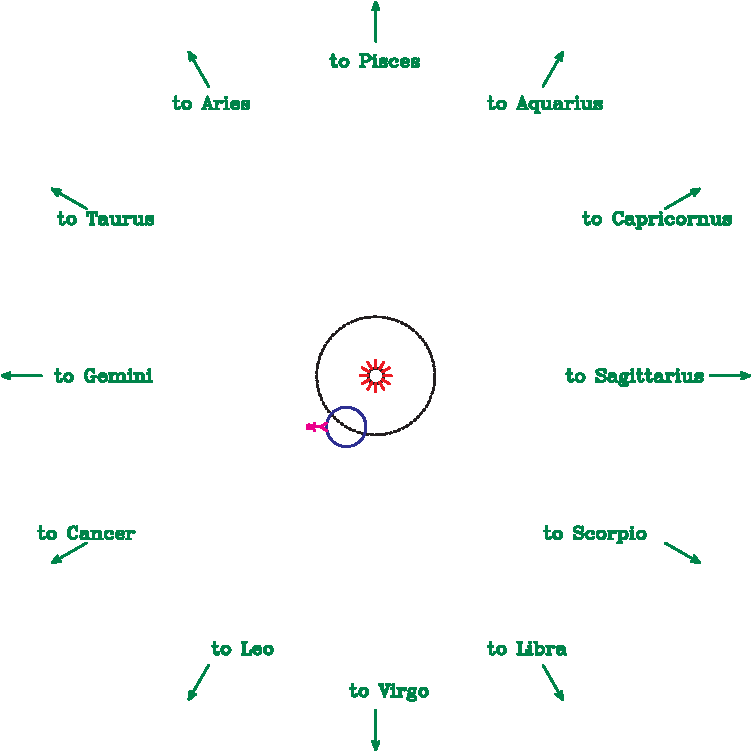
\includegraphics [width=0.8\textwidth]{hw-diagram-crop.pdf}
\end{center}


\begin{enumerate}
	

	\item What time of day is it for our observer? (Give a general answer: noon, midnight, just before sunset, just after sunrise, etc.)
	\vspace{1em}


\item Draw the horizon line for the observer, keeping in mind that the Earth is really a lot smaller than shown.

	\item What constellation is highest in the sky for our observer at this time?
	
	\vspace{0.5in}
	
	\item How much time would the observer need to wait to see the constellation Libra? (Give a general answer: a few hours, a day, a month, etc.) What needs to happen before they can see it?
	
	\vspace{0.8in}
	
	\item How much time would the observer need to wait to see the constellation Aquarius? (Give a general answer: a few hours, a day, a month, etc.) What needs to happen before they can see it?
	
	\vspace{0.8in}
	
	\item In astrology, the ``sun sign'' of a particular time of year refers to the constellation that is lined up with the Sun as seen from Earth. It is mid-December, when the Sun is lined up with Sagittarius. Two star-watchers, Sybill and Neil, are having a debate:
	
	{\bf Sybill:} It's December. So I should expect the ``winter signs'', like Sagittarius, to be highest in the sky at midnight.
	
	{\bf Neil:} No, it's the other way around. If Sagittarius is lined up with the Sun in December, you'd have to wait six months later to see it high in the sky at midnight. In December you expect to see the ones on the other side of the sky, like Gemini, high in the sky at midnight.
	
	Who is right and why?
	
\end{enumerate}
\begin{center} \underline {\hspace{4in}} \end{center}
The homework quiz for this homework will be Thursday, September 15. On it I will give you the chart on the first page, with the Earth drawn at a particular position.

I will ask you:

\begin{enumerate}
	\item To draw me a stick figure on the Earth corresponding to a particular time of day
	
	\item What constellations that observer can see, where they would be in the sky, and what constellation is behind the Sun at that time
	
	\item What constellations the observer would see a certain amount of time later, and where they would be in the sky
	
	\item How long the observer would have to wait to see something happen in the sky (like questions 4 and 5)


\end{enumerate}





\end{document}

